\documentclass[]{final_report}
\usepackage{graphicx}
\usepackage{hyperref}
\usepackage{caption}
\usepackage[backend=bibtex]{biblatex}
%\bibliography{report_template.bib}
\setcounter{tocdepth}{3}

%%%%%%%%%%%%%%%%%%%%%%
%%% Input project details
\def\studentname{John Patrick Bracken}
\def\projecttitle{Reputation Algorithms for the Social Web}
\def\supervisorname{Dr. Michael O'Mahony}
%\def\moderatorname{}
\def\stack{Stack Exchange}


\begin{document}

\maketitle
\tableofcontents\pdfbookmark[0]{Table of Contents}{toc}\newpage

\begin{specification}

\textbf{\textsl{Subject:}} Social Network Analysis, Reputation Systems

\textbf{\textsl{Prerequisites:}} None

\textbf{\textsl{Corequisites:}} None

\textbf{\textsl{Coverage}} Social Network Analysis, Reputation Systems

\textbf{\textsl{Project Type:}} Design and Implementation

\textbf{\textsl{Software Requirements:}} Java, Linux, MySQL (or other)

\textbf{\textsl{Hardware Requirements:}} Laptop for development. Access to server will be provided if necessary.

\textbf{\textsl{Preassigned:}} No


\textbf{Description}
\textsl{General Information:}

The social web reflects an important paradigm shift in the nature of our online transactions. We increasingly rely on the opinions of others to mediate these transactions and as such the reliability of these users becomes an important indicator of quality. Thus, the concept of user reputation has become increasingly important in the context of today's social web. Recently, there has been considerable research on various approaches to model the reputation of users as they participate in a diverse array of online interactions.

The goal of this project is to design, implement and evaluate reputation algorithms for users of the Stack Exchange network, a popular group of social Q\&A sites. There are currently over 80 topical Stack Exchange websites, hosting almost 2 million users. Some 3.8 million questions have been posed, eliciting 7.7 million answers. Users are permitted to post questions that can be answered by other users in the community. Each answer given can be voted up or down by others and the questioner can chose to highlight a single answer as correct, indicating the question has been answered satisfactorily or that answer was the best answer provided. The availability of such data can be leveraged to estimate the reputation of users; for example, if the answers provided by a particular user are frequently deemed to be correct and/or receive many positive votes from the community, then this provides an indication that the user is knowledgeable about particular subject matters.

\textbf{Mandatory:}
\begin{itemize}
\item Download Stack Exchange data (http://data.stackexchange.com/) - data from three sites should be obtained.
\item Implementation of reputation algorithms from the literature.
\item Evaluation: for each dataset, compare the performance of these algorithms to the user reputation model currently used on Stack Exchange.
\end{itemize}

\textbf{Discretionary:}
\begin{itemize}
\item Predict the correct answers to questions based on user reputation.
\item Evaluate the accuracy of predicted answers.
\item Perform user-trials and correlate prediction performance with offline metrics.
\end{itemize}

\textbf{Exceptional:}

Any (but not limited to) the following:

\begin{itemize}
\item Propose and implement enhancements to improve algorithm performance.
\item Analyse the robustness of the reputation algorithms against attack.
\end{itemize}

\textbf{Reading:}
\begin{itemize}
\item Stack Exchange: http://stackexchange.com/
\item Stack Exchange Data Explorer: http://data.stackexchange.com/
\item A Model of Collaboration-based Reputation for the Social Web – ICWSM 2013 
\item Trust Among Strangers in Internet Transactions: Empirical Analysis of eBay’s Reputation System - Advances in Applied Microeconomics 2012 (attached)
\end{itemize}
\end{specification}

%%%%%%%%%%%%%%%%%%%%%%
%%% Your Abstract herebstract

% TODO: Remove hard embedded date from cls file

\begin{abstract}

In this project I intend to compare the performance of generic reputation algorithms using the Stack Exchange Question and Answer sites' open-sourced data dumps. These algorithms will include a simple inbound weighted sum, Page and Brin's PageRank, and Kleinburg's Hubs and Authorities algorithm. Performance will be analysed by evaluating correlation between these algorithms scores and the bespoke Stack Exchange reputation model.

I will also attempt to predict the correct answers to questions using user reputation scores, and perform user trials on Q\&A data.

\end{abstract}
\newpage

\chapter*{Acknowledgments}

%%%%%%%%%%%%%%%%%%%%%%
%%% Introduction

\chapter{Introduction}

With the increasing use of the internet in our day-to-day tasks, it has become more and more important that we be able to verify the trustworthiness of the strangers we so often rely on. While the use of technologies such as public key encryption allow us to verify \textsl{who} we are talking to with reasonable confidence, we are still left with the problem of determining that person's trustworthiness as an individual---whether that be trust in their knowledge in a particular field, or that they can be relied upon to deliver a good or service to satisfaction.

To that end there has been considerable recent research into the fields of peer-to-peer trust and user reputation systems in social networks (McNally, O'Mahony and Smyth 2013; Cheng and Vassileva 2005; Mui 2002).

There are numerous contexts in which an indication of trust may be desired online, from internet transactions to Question \& Answer sites. For the purposes of this project we will be focusing on the exchange of knowledge and expertise between users on the \textsl{Stack Exchange Question and Answer} network. We will define trust as a relationship between users, and reputation will refer to an aggregate score allocated to a user that reflects their trustworthiness.

In this project, I will be implementing a number of generic approaches to reputation (Weighted Sum; Hubs and Authorities, or HITS; and PageRank) and comparing their performance on the Stack Exchange datasets to each other and to the Stack Exchange ad-hoc reputation model.

To demonstrate the necessity for these reputation modelling, it is important to pay attention to the history of the Web up to its present state, and to look at current trends to predict its future.

When the web first exploded into widespread use in the nineties, it was a static compilation of pages connected by hyper links. Typically, websites were only published by universities, government organisations and corporations, with content being controlled by their respective web-masters. It was much easier, then, to evaluate the trustworthiness of online resources; content related to hardware published by IBM was likely to be accurate, but IBM's advice on cake-baking may be taken with a pinch of salt (or perhaps not).

Over time however, computers became more sophisticated, and so-called web 2.0 technologies such as PHP and JavaScript evolved which allowed end-users to interact dynamically with the web. At the same time, the number of internet users exploded, and the line between the roles of producer and consumer began to blur. Instead, anyone could post on a social network, publish a music review to potentially millions of people, or share crude comments on YouTube videos.

In many cases this is not an issue, as many of these forms of communication are entirely--and transparently--opinion based. But there are increasingly more cases these days where it is beneficial to know if another person should be trusted.

To give an example, Alice asks a dog lovers' web-forum how much chocolate is safe to feed to her chihuahua Charlie. She may get a range of different answers. Bob helpfully gives her the correct answer that chocolate is bad for humans and worse for dogs, and to feed Charlie treats made especially for dogs instead. Mallory, out of some sense of bizarre Schadenfreude, intentionally gives her a malicious answer framed as genuine advice. Alice does not know who to trust, but errs on the side of caution and Charlie is spared the grim fate of diabetes.

Not all negatively impactful users are malicious. Some users may just be misinformed, or have the illusory superiority cognitive bias, in which a person overestimates their own abilities or knowledge (Hoorens 1993).

While the above example is contrived, it illustrates the potential dangers of this social web. Credulous users may take inaccurate information at face value, and in the worst case cause themselves or others serious harm, due to the maliciousness or ignorance of a stranger.

With over a billion active users and more than ten billion messages every day on Facebook \textsl{alone}\footnote{Some figures taken from presentation 'A focus on Efficiency' by Facebook, Ericsson and Qualcomm 2013 (internet.org, September 16, 2013)}, for example, there is a considerable amount of potentially inaccurate information being spread social networks, and it would be nice to be able to filter some of the what from the chaff.

This filtering of unsatisfactory content can take many different forms. Favourable content may 'rise to the top' of a user's news feed in order of best to worst. Negative content might be given some visual de-emphasis to indicate its lower quality, or may even be hidden from the user altogether. Users might be able to customize how strict this filtering is, or create whitelists and blacklists of people they trust and distrust respectively.

In chapter 2, I describe some reputation algorithms at a high level, and present three case studies of reputation systems used online.



\chapter{Background Research (10 pages)}

\section{Introduction}

In the following chapter I outline the research I have undertaken so far on online reputation systems.

I define trust and reputation, and briefly explain their differences and why drawing a distinction between the two is important. I  briefly describe the user reputation algorithms that are currently in use across the web, and go into further detail on the algorithms I will be evaluating. Finally,  I will present a number of case studies on sites that use a user reputation model, such as the Stack Exchange Network, eBay and Klout.


\section{Trust and Reputation}

For the purposes of this project, \textsl{trust} is defined as a relationship between two parties. A trustor is an entity who places a certain amount of faith in the actions or knowledge of another entity, (or the trustee). Trust is not a symmetric relationship, so while, for example, a student may trust a teacher's knowledge in their subject matter, the teacher will likely have less (or no) trust in their student's knowledge  (McNally, O'Mahony and Smyth 2013).

Trust can occur between numerous types of entities, such as between people or web-pages (Page, L., Brin S., Motwani, R., and Winograd, T. 1999). It is inherently a difficult property to quantify in any accurate way, and is why the need to draw a distinction between \textsl{trust} and \textsl{reputation} arises.

For the purposes of this paper, \textsl{reputation} is defined as a numeric measure of a user's \textsl{trustworthiness} according to some metric performed on their individual trust scores (McNally, O'Mahony and Smyth 2013).

There are a number of generic and ad-hoc implementation across the web. Examples of these are Google's PageRank algorithm for measuring a web-page's importance, Stack Exchange's system based on user activity, or eBay's implementation which uses user reviews to calculate reputation. Many of these implementations are bespoke systems, designed especially for their domain.


\section{Reputation Algorithms}
In the following section I discuss a number of ways that reputation can be measured. In these techniques the term producer refers to a creator of content, consumer to the person who receives that content, and score is a number awarded to the producer for that content.

%\subsection{Weighted Sum}
%Description of Weighted Sum.
%\subsection{PageRank}
%Words go here.
%\subsection{Hubs and Authorities}
%Words go here.
\section{Case studies}

In this section I present case studies for three bespoke user reputation models. The activity-based Stack Exchange model, eBay's user-feedback centric reputation model and Klout's social network influence reputation model.

\subsection{Stack Exchange -- An activity based approach}

The Stack Exchange network\footnote{http://stackexchange.com/} is a collection of Question and Answer (Q\&A) communities, each focused on a specific field of expertise, with a site for everything from programming to bicycling and cooking. The network grew from the original Stack Overflow site, which focused on computer programming questions, and it currently still the largest site in the network. As of the time of writing this report, the network consists of 114 Q\&A sites, almost 4.5 million users and over 8 million questions with 14.6 million answers.

\begin{figure}[ht!]
\centering
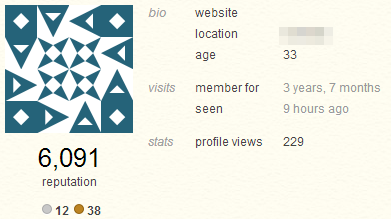
\includegraphics[width=100mm]{serep.png}
\caption{A cooking.stackexchange.com profile, showing reputation score.}
\end{figure}


The Stack Exchange network uses a bespoke model of reputation. A user's reputation is calculated as a sum of points earned by contributing to the sites in various ways. Nearly every site activity, from asking and answering questions, to suggesting edits and flagging content for moderation, can earn the user reputation points. This system is aimed more towards encouraging site activity than accurately evaluating a user's trust. A user can theoretically gain a considerable amount of reputation without actually demonstrating any domain knowledge.

\begin{minipage}{\linewidth}
\centering
\begin{tabular}{|l|l|}
\hline \textbf{Site activity} & \textbf{Reputation reward} \\ 
\hline Your question voted up & +5 \\ 
\hline Your answer voted up & +10 \\ 
\hline Your answer 'accepted' as correct & +15 \\ 
\hline You 'accept' an answer to your own question & +2 \\ 
\hline Your suggested edit accepted & +2 (up to a total of 1000) \\ 
\hline 
\end{tabular}\par
\captionof{table}{Stack Exchange reputation rewards} \label{tab:title}
\end{minipage}


Additionally, reputation can be lost for a number of reasons, ranging from abuse of the site, to low-quality submissions, although reputation never falls below 1. Moderation is largely performed by the community itself, as increasing reputation scores are rewarded with additional site privileges, ranging from moderation tools to access to chat-rooms.


\subsection{eBay -- A feedback-based approach}

eBay Inc. is an online auction-house and market-place based entirely around user-to-user transactions. Originally founded in 1995, it has seen steady growth since, and has become the world's largest online marketplace, with over 112 million active users and \$175 billion USD worth of transactions facilitated by the site in 2012 alone.

With such a large volume of transactions passing through the site, evaluating trust is one of eBay's principle concerns. eBay calculates reputation using user feedback after transactions. For each positive transaction, the user's reputation score is increased by one point. If they receive neutral feedback, there is no change to their reputation, and if a transaction receives negative feedback, the user's reputation is decreased by one point.

In the event that there are multiple transactions between users in a single week, eBay aggregates the reputation points the user would have received. If this number is then positive, the reputation score is increased by one, if it is neutral, it does not change, and if it is negative, they lose one reputation point.

As a user's feedback score grows, they gain a coloured star next to their display name as a quick visual indicator of their reputation. Sellers who consistently gain lots of positive feedback and make frequent sales can also gain a 'top-rated seller' badge that informs buyers that they consistently provide good service\footnote{Information taken from 'How feedback works'. Available at http://pages.ebay.co.uk/help/feedback/howitworks.html, last accessed 10th February 2014.}.

Additionally, users can leave reviews with their feedback, where they may describe their interactions with the seller, the quality of the product, and the cost and speed of shipping.

\begin{figure}[ht!]
\centering
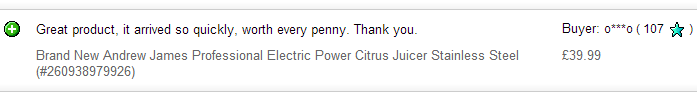
\includegraphics[width=140mm]{ebayfeedback.png}
\caption{An example of eBay feedback}
\end{figure}

This combination of easy to understand reputation score and collection of user reviews allows buyers to quickly find trustworthy sellers and decide from which of them they wish to conduct their business.

\subsection{Klout}

Klout is an online service and mobile application that attempts to measure a user's \textsl{influence} across social networks. Launched in 2008, it uses analytics from eight different social media websites to evaluate its users' reputation scores, which they call the \textsl{Klout Score}. This reputation score is an integer value bounded between 1 and 100, and becomes increasingly difficult to improve upon as it increases\footnote{http://klout.com/corp/about and http://klout.com/corp/score}.

Among the metrics Klout uses to determine reputation are activity from Twitter, Facebook, the user's Wikipedia page (if they are fortunate enough to have one), Google+ and others. When a user produces content on these sites that gains 'likes', generates discussion or is shared with others, Klout deems that this content generates \textsl{influence} to a lesser or greater degree, and so affects their reputation.

\begin{figure}[ht!]
\centering
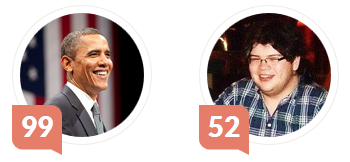
\includegraphics[width=80mm]{klout.png}
\caption{Barack Obama is considerably more reputable than I am.}
\end{figure}

Although Klout does not specify exactly how it calculates reputation, there is evidence that the algorithms used on these \textsl{signals} or \textsl{collaboration events} are actually quite simple. In June, 2011, a Ph.D candidate in Montana State University, Sean Golliher, managed to calculate Klout's reputation score with an accuracy of 94\% simply by calculating a logarithm of the number of a user's followers and retweets\footnote{http://www.seangolliher.com/2011/uncategorized/how-i-reversed-engineered-klout-score-to-an-r2-094/}.

\section{Conclusion}

\chapter{Main Chapter (8 Pages)}

\chapter{Design \& Implementation (5 Pages)}

\chapter{Testing \& Evaluation (8 Pages)}

\chapter{Conclusions \& Future Work}

%%%% ADD YOUR BIBLIOGRAPHY HERE
\newpage
\raggedright
\textbf{McNally, K., O'Mahony, M.P., and Smyth, B. 2013} -- A Model of Collaboration-based Reputation for the Social Web
\linebreak
\linebreak
\textbf{Cheng, R., and Vassileva, J. 2005} -- Reward Mechanism for Sustainable Online Learning Community. In Proceedings of the 2005 conference on Artificial Intelligence in Education. IOS Press.
\linebreak
\linebreak
\textbf{Page, L., Brin S., Motwani, R., and Winograd, T. 1999} -- The PageRank citation ranking: Bringing order to the Web.
\linebreak
\linebreak
\textbf{Mui, L. 2002} -- A Computational Model of Trust and Reputation. Agents, Evolutionary Games, and Social Networks
\linebreak
\linebreak
\textbf{Resnick, P., and Zeckhauser, R. 2002} -- Trust Among Strangers in Internet Transactions: Empirical Analysis of eBay's Reputation System. Advances in Applied Microeconomics 11:127?157
\linebreak
\linebreak
\textbf{Gyongyi, Z., Garcia-Molina, H., Pedersen, J.} -- Combating Web Spam with TrustRank
\linebreak
\linebreak
\textbf{Massa, P., Avesani, P. 2007} -- Trust-Aware Recommender Systems
\linebreak
\linebreak
\textbf{Hoorens, Vera} -- Self-enhancement and Superiority Biases in Social Comparison. The European Review of Social Psychology (1993), Volume 4, Issue 1 p113-139

%\begin{thebibliography}{99}


%\end{thebibliography}
\label{endpage}

\end{document}

\end{article}
